\documentclass[11pt]{article}
\usepackage[margin=0.75in]{geometry}
\usepackage{setspace}
\usepackage{amsmath}
\usepackage{booktabs}
\usepackage{tabularx}
\usepackage{hyperref}
\usepackage{graphicx}
\hypersetup{colorlinks=true, allcolors=black}
\setlength{\parindent}{0pt}
\setlength{\parskip}{0.35em}
\setstretch{1.05}
\pagestyle{empty}
\usepackage{titlesec}
\titlespacing*{\section}{0pt}{0.6em}{0.3em}
\titlespacing*{\subsection}{0pt}{0.5em}{0.2em}

\begin{document}

\begin{center}
{\Large Evidence of Teaching Effectiveness}\\[0.4em]
HSU Ke Cheng\\
Ph.D.\ Candidate in Economics\\[0.2em]
{\small Email: \href{mailto:khsu@connect.ust.hk}{khsu@connect.ust.hk}
\quad Website: \href{https://cliohsu1997.github.io/}{cliohsu1997.github.io}}
\end{center}

I served as a Teaching Assistant at the Hong Kong University of Science and Technology from 2020 to 2025. All scores are on a 1--5 scale. Across the five teaching-assistant appointments listed below, from the earliest to the latest, my average evaluation is \textbf{4.72 out of 5}. My evaluation as instructor of the MSc Economics Math Bootcamp is reported separately at the end.

\section*{1.\ Teaching assistant appointments}

The first three appointments used one questionnaire and were reported on a 0--100 scale. I transform each adjusted mean \(x\) to a 1--5 scale by \(1 + x/25\), so that 0 corresponds to 1 and 100 corresponds to 5. The two ECON 5210 appointments used a different questionnaire and were already reported on a 1--5 scale; I use the adjusted mean. Each item below is then the average across the appointments that included it.

{\small
\begin{tabularx}{\textwidth}{@{}X c@{}}
\toprule
& Average \\
\midrule
\multicolumn{2}{@{}l}{\emph{ECON 4999T, ECON 2123, and ECON 4134}} \\
The TA is approachable and friendly. & 4.76 \\
The TA is responsive to my requests. & 4.67 \\
The TA provides accurate and timely information. & 4.76 \\
The TA proactively reminds me of key dates and activities. & 4.80 \\
The TA serves as an effective bridge with the professor. & 4.48 \\
Are you satisfied with your TA? & 4.53 \\
Is your TA helpful in general? & 4.47 \\
\midrule
\multicolumn{2}{@{}l}{\emph{ECON 5210, 2023--24 Fall and 2024--25 Fall}} \\
Tutorial materials and activities helped me achieve the learning outcomes. & 4.85 \\
The TA was good at explaining things to me. & 4.83 \\
The TA encouraged me to participate actively. & 4.83 \\
The TA provided informative and constructive answers. & 4.82 \\
The TA was readily available outside tutorial classes. & 4.82 \\
The TA provided helpful and timely feedback. & 4.85 \\
Overall, I am satisfied with the teaching and assistance provided by the TA. & 4.84 \\
Overall, I am satisfied with the tutorial sections. & 4.83 \\
\midrule
Average across the five appointments & 4.72 \\
\bottomrule
\end{tabularx}
}

\section*{2.\ Instructor evaluation: MSc Economics Math Bootcamp (2026)}

{\small
\begin{tabularx}{\textwidth}{@{}X c@{}}
\toprule
& Mean \\
\midrule
The objectives and expectations were clearly communicated. & 4.40 \\
The content was relevant to my preparation. & 4.38 \\
The bootcamp strengthened my understanding of key mathematical concepts. & 4.36 \\
The bootcamp increased my confidence in applying mathematical concepts. & 4.02 \\
The teaching materials, exercises, and learning activities were useful. & 4.40 \\
The level and pace were appropriate for my background. & 4.08 \\
Overall, I am satisfied with the Math Bootcamp. & 4.38 \\
\midrule
Average of course items & 4.29 \\
\bottomrule
\end{tabularx}
}

The two lower scores, on whether the bootcamp increased confidence in applying mathematical concepts (4.02) and whether the level and pace were appropriate for students' backgrounds (4.08), reflect the design of the course. Many students came from non-mathematics backgrounds, and the bootcamp covered optimization, linear algebra, real analysis, calculus, and dynamic programming in five days.

\vspace{0.4em}
{\small
\begin{tabularx}{\textwidth}{@{}X c@{}}
\toprule
& Mean \\
\midrule
The instructor explained concepts clearly and effectively. & 4.43 \\
The instructor encouraged participation and created a supportive learning environment. & 4.55 \\
The instructor was well prepared and responsive to students' questions. & 4.64 \\
Overall, I am satisfied with the teaching and support provided by the instructor. & 4.51 \\
\midrule
Average of instructor items & 4.53 \\
\bottomrule
\end{tabularx}
}

\clearpage
\thispagestyle{empty}
\begin{center}
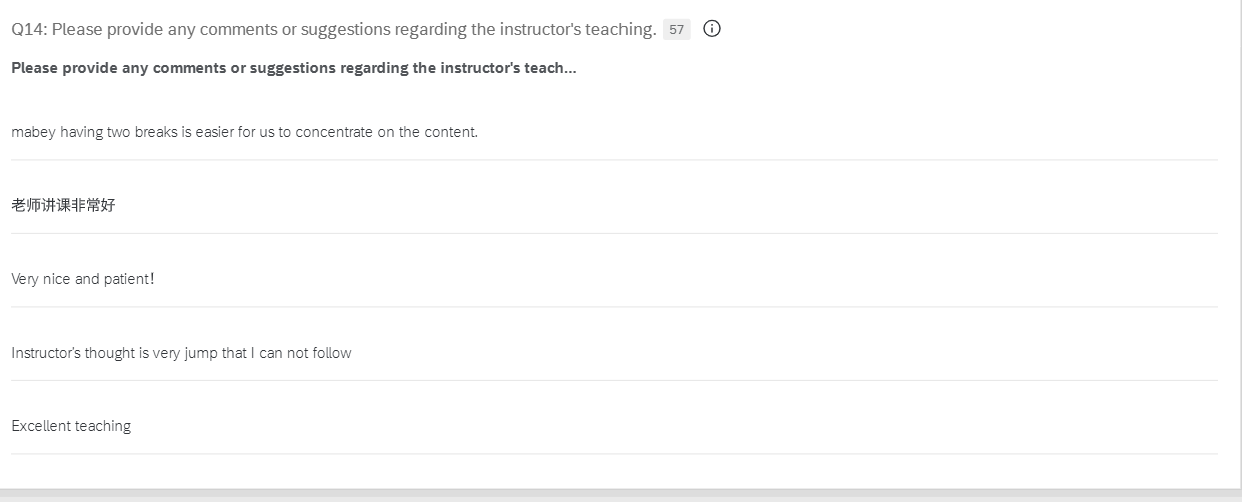
\includegraphics[width=\textwidth]{teaching_report/msc_instructor_comments_Q14.png}
\end{center}

\end{document}
